\documentclass[11pt,a4paper]{article}

% ====================== PAKIETY ======================
\usepackage[utf8]{inputenc}
\usepackage[T1]{fontenc}
\usepackage[polish]{babel}
\usepackage[a4paper,margin=2.3cm]{geometry}
\usepackage{lmodern}
\usepackage{graphicx}
\usepackage{array}
\usepackage{longtable}
\usepackage{booktabs}
\usepackage{tabularx}
\usepackage{enumitem}
\usepackage{xcolor}
\usepackage{titlesec}
\usepackage{fancyhdr}
\usepackage{tikz}
\usepackage{float}
\usetikzlibrary{shapes.geometric, shapes.multipart, arrows.meta, positioning, fit, backgrounds, calc}
\usepackage[hidelinks]{hyperref}
\usepackage{caption}
\usepackage{placeins}

% ====================== KOLORY ======================
\definecolor{primary}{RGB}{30,90,150}
\definecolor{accent}{RGB}{0,140,120}
\definecolor{lightgray}{RGB}{240,242,245}
\definecolor{midgray}{RGB}{170,178,186}
\definecolor{ucfill}{RGB}{225,238,248}
\definecolor{compfill}{RGB}{235,245,238}

% ====================== STYLE NAGŁÓWKÓW ======================
\titleformat{\section}{\normalfont\Large\bfseries\color{primary}}{\thesection.}{0.6em}{}
\titleformat{\subsection}{\normalfont\large\bfseries\color{accent}}{\thesubsection}{0.6em}{}
\titlespacing*{\section}{0pt}{18pt}{8pt}

% ====================== STOPKA / NAGŁÓWEK ======================
\pagestyle{fancy}
\fancyhf{}
\renewcommand{\headrulewidth}{0.4pt}
\renewcommand{\footrulewidth}{0.4pt}
\fancyhead[L]{\small\color{primary}\textbf{Tripify}}
\fancyhead[R]{\small Dokument Architektury}
\fancyfoot[L]{\small Politechnika Łódzka}
\fancyfoot[R]{\small Strona \thepage}

% ====================== POMOCNICZE ======================
\newcolumntype{Y}{>{\raggedright\arraybackslash}X}
\newcommand{\sysname}{\textbf{Tripify}}
\setlist{itemsep=2pt, topsep=3pt}

% ---- Style diagramów ----
\tikzset{
  layer/.style={rectangle, rounded corners, draw=primary, thick, fill=lightgray,
                minimum width=3.4cm, minimum height=1cm, align=center, font=\small},
  ext/.style={rectangle, rounded corners, draw=accent, thick, fill=white,
              minimum width=2.8cm, minimum height=0.9cm, align=center, font=\small},
  arr/.style={-{Stealth[length=3mm]}, thick, draw=primary!70},
  uc/.style={ellipse, draw=primary, thick, fill=ucfill, align=center,
             font=\scriptsize, minimum width=2.9cm, minimum height=0.95cm, inner sep=2pt},
  comp/.style={rectangle, draw=accent, thick, fill=compfill, rounded corners=2pt,
               align=center, font=\scriptsize\bfseries, minimum width=2.7cm, minimum height=1cm},
  cls/.style={draw=primary, thick, fill=lightgray, rectangle split,
              rectangle split parts=2, font=\scriptsize, text width=3.0cm,
              align=left, rounded corners=2pt},
  part/.style={draw=primary, thick, fill=lightgray, rounded corners,
               minimum width=2.5cm, minimum height=0.8cm, font=\footnotesize\bfseries, align=center},
}
% Aktor (stick figure) jako pic
\tikzset{actorpic/.pic={
  \draw[thick] (0,0) circle (3.2mm);
  \draw[thick] (0,-3.2mm) -- (0,-12mm);
  \draw[thick] (-5mm,-7mm) -- (5mm,-7mm);
  \draw[thick] (0,-12mm) -- (-5mm,-20mm);
  \draw[thick] (0,-12mm) -- (5mm,-20mm);
}}
\tikzset{systempic/.pic={
  \draw[thick] (0,0) -- (-0.25, 0.15) -- (-0.25, 0.45) -- (0, 0.6) -- (0.25, 0.45) -- (0.25, 0.15) -- cycle; 
  \draw[thick] (0,0) -- (0, 0.3); 
  \draw[thick] (-0.25, 0.45) -- (0, 0.3) -- (0.25, 0.45); 
  \draw[thick] (0,0) -- (0,-0.6);
  \draw[thick] (-0.4,0) -- (0.4,0);
  \draw[thick] (-0.3,-1) -- (0,-0.6) -- (0.3,-1);
}}

% Wiadomości w diagramach sekwencji
\newcommand{\msg}[4]{\draw[-{Stealth[length=2mm]},thick,primary] (#1 |- 0,#3) -- node[above,font=\scriptsize,midway,text=black]{#4} (#2 |- 0,#3);}
\newcommand{\rsg}[4]{\draw[-{Stealth[length=2mm]},dashed,accent] (#1 |- 0,#3) -- node[above,font=\scriptsize,midway,text=black]{#4} (#2 |- 0,#3);}

\begin{document}

% ====================== STRONA TYTUŁOWA ======================
\begin{titlepage}
\centering
\vspace*{2cm}
{\Huge\bfseries\color{primary} Dokumentacja\par}
\vspace{0.5cm}
{\LARGE Inteligentny planer podróży\par}
\vspace{0.3cm}
{\Huge\bfseries Tripify\par}
\vspace{1.2cm}
\rule{0.7\textwidth}{1.2pt}\par
\vspace{1.2cm}
{\large\textbf{Instytucja:} Politechnika Łódzka\par}
\vspace{0.4cm}
{\large\textbf{Data:} 23 czerwca 2026\par}
\end{titlepage}

% ====================== LISTA CZŁONKÓW ZESPOŁU ======================
\section*{Lista członków zespołu}
\addcontentsline{toc}{section}{Lista członków zespołu}
\begin{table}[ht]
\centering
\begin{tabularx}{\textwidth}{>{\bfseries}p{4.2cm} p{3.5cm} Y}
\toprule
\textbf{Imię i nazwisko} & \textbf{Rola} & \textbf{Obszar} \\
\midrule
Kacper Błaszczyk & Project Manager & Koordynacja, architektura, wymagania. \\
Klim Hudzenko & Backend Developer & Backend (FastAPI), baza danych, API. \\
Maciej Miazek & Frontend Developer & Frontend (Next.js), integracje. \\
Remigiusz Tomecki & Frontend Developer & Frontend (Next.js), interfejs użytkownika. \\
Kacper Romek & Tester & Testy, zapewnienie jakości. \\
\bottomrule
\end{tabularx}
\caption{Skład zespołu projektowego RehabSense.}
\end{table}
\newpage

% ====================== SPIS TREŚCI ======================
\tableofcontents
\newpage

% ====================================================
\section{Wprowadzenie}
% ====================================================
\subsection{Cel dokumentu}
Niniejszy dokument przedstawia architekturę systemu \sysname{}. Opisuje przeznaczenie i funkcje oprogramowania, kluczowe przypadki użycia (wraz ze scenariuszami), strukturę komponentów mikrousługowych, model danych (diagram klas) oraz interakcje między elementami systemu (diagramy sekwencji). Celem dokumentu jest dostarczenie spójnego rozwiązania, stanowiącego podstawę implementacji, testów i dalszego rozwoju.

\subsection{Zakres projektu}
\sysname{} to nowoczesna aplikacja webowa do inteligentnego planowania podróży. Dzięki wykorzystaniu sztucznej inteligencji (modele LLM), system automatycznie generuje spersonalizowane plany wycieczek na podstawie preferencji użytkownika. Dodatkowo integruje informacje o aktualnej pogodzie w miejscach docelowych, dostarcza zdjęcia lokalizacji oraz zawiera moduł przeliczania walut w czasie rzeczywistym. Projekt zrealizowano w skalowalnej architekturze mikrousług.

\subsection{Odbiorcy projektu}
\begin{itemize}
  \item \textbf{Podróżujący} — osoby poszukujące zautomatyzowanego wsparcia w układaniu planów podróży.
  \item \textbf{Deweloperzy} — twórcy wykorzystujący funkcjonalności naszego systemu
\end{itemize}

% ====================================================
\section{Opis testowanego systemu}
% ====================================================
\subsection{Przeznaczenie oprogramowania}
\sysname{} to narzędzie zwalniające użytkownika ze żmudnego procesu organizowania harmonogramu wycieczki. Oprogramowanie wykorzystuje algorytmy sztucznej inteligencji, aby rekomendować lokalizacje ,,must-see'' oraz integruje kluczowe dane z punktu widzenia podróżnika (pogoda, kursy walut).

\subsection{Główne funkcje aktorów systemu}
\begin{itemize}
  \item \textbf{Użytkownik:} Rejestracja i logowanie (w standardzie OAuth2), definiowanie celu i parametrów podróży, przeglądanie wygenerowanego planu, sprawdzanie pogody i zdjęć miejsc, kalkulator walutowy.
  \item \textbf{Zewnętrzne API (System):} Model LLM generujący plan wycieczki, usługi dostarczające dane pogodowe, kursy wymiany walut i obrazy z miejsc docelowych.
\end{itemize}

\subsection{Architektura systemu}
System zbudowano zgodnie z architekturą \textbf{Mikrousług}. Obejmuje wiele niezależnych, ale ściśle współpracujących komponentów. Frontend w React.js/Next.js komunikuje się poprzez centralny \texttt{API Gateway} z usługami back-endowymi napisanymi w Javie (Spring Boot) oraz Go. Za autoryzację odpowiada dedykowany \texttt{Auth Server}, a zarządzanie siecią i konfiguracją realizują \texttt{Eureka Server} oraz \texttt{Config Server}. Dane gromadzone są w chmurowej bazie PostgreSQL.

\begin{figure}[H]
\centering
\begin{tikzpicture}
% Zwiększone odstępy poziome i pionowe, aby bloki miały więcej "oddechu"
\node[layer] (front) at (0, 2.5) {\textbf{Warstwa Prezentacji}\\ Frontend (Next.js)};
\node[layer] (gateway) at (0, 0) {\textbf{API Gateway}\\ Główny router (Spring)};
\node[layer] (infra) at (5.5, 1.5) {\textbf{Infrastruktura}\\ Eureka \& Config Server};

\node[layer] (auth) at (-5.0, -2.5) {\textbf{Auth Server}\\ OAuth2 \& JWT};
\node[layer] (ai) at (0, -2.5) {\textbf{AI Service}\\ Groq LLM (Spring)};
\node[layer] (curr) at (5.0, -2.5) {\textbf{Currency Conv.}\\ Golang z cache};

\node[layer] (db) at (0, -6.5) {\textbf{Warstwa Danych}\\ Cloud SQL (PostgreSQL)};
\node[ext] (ext) at (5.0, -6.5) {\textbf{API Zewnętrzne}\\ OpenWeather, Unsplash, NBP};

% Główne przepływy od API Gateway
\draw[arr] (front) -- (gateway);
\draw[arr] (gateway.west) -| (auth.north);
\draw[arr] (gateway.south) -- (ai.north);
\draw[arr] (gateway.east) -| (curr.north);

\draw[arr] (auth.south) |- (db.west);
\draw[arr] (ai.south) -- (db.north);
\draw[arr] (ai.east) -- ++(1.0,0) -- ++(0,-1.5) -| ([xshift=-1.0cm]ext.north);

\draw[arr] (curr.south) -- (ext.north);

% Service Discovery (linia nie będzie już nachodzić na inne ścieżki)
\draw[arr, dashed] (infra.west) -| node[above left, font=\scriptsize] {Service Discovery} (gateway.north east);
\end{tikzpicture}
\caption{Architektura mikrousług systemu Tripify.}
\end{figure}

\subsection{Integracje z systemami zewnętrznymi}
\begin{itemize}
  \item \textbf{Groq API} — API obsługujące modele LLM do generowania planów wycieczek.
  \item \textbf{Unsplash API} — pobieranie dynamicznych, estetycznych zdjęć dla miast i państw.
  \item \textbf{OpenWeather API} — aktualne prognozy pogodowe wykorzystywane w planowaniu.
  \item \textbf{NBP API} — zapewnia kursy walut
  \item \textbf{Google Cloud SQL} — rozwiązanie typu PaaS do hostowania bazy PostgreSQL.
\end{itemize}

\newpage
% ====================================================
\section{Diagramy przypadków użycia}
% ====================================================
Poniższy diagram przedstawia główne przypadki użycia w systemie.

\begin{figure}[H]
\centering
\resizebox{0.98\textwidth}{!}{%
\begin{tikzpicture}

% Granica systemu
\draw[thick] (-5.5, -6.5) rectangle (12, 6.5);
\draw[thick, fill=white] (-5.5, 6.5) -- (-5.5, 7.3) -- (-2.5, 7.3) -- (-2.2, 6.5) -- cycle;
\node[font=\bfseries, right] at (-5.3, 6.9) {Tripify};

% ========== Przypadki użycia — Użytkownik (lewa/centralna strona) ==========

% Grupa: Uwierzytelnianie
\node[uc, minimum width=3.2cm] (logowanie)   at (0.0, 5.0) {Logowanie / Rejestracja};

% Grupa: Planowanie podróży
\node[uc, minimum width=3.2cm] (generowanie)  at (0.5, 3.0)  {Generowanie planu \\ wycieczki przez AI};
\node[uc, minimum width=3.2cm] (widokplanu)   at (0.5, 1.0) {Przeglądanie \\ wygenerowanego planu};

% Grupa: Zarządzanie planami
\node[uc, minimum width=3.2cm] (zapis)        at (0.0, -1.0) {Zapisywanie planu \\ do bazy danych};
\node[uc, minimum width=3.2cm] (historia)     at (0.0, -3.0) {Przeglądanie historii \\ planów podróży};

% Grupa: Waluta
\node[uc, minimum width=3.2cm] (waluty)       at (0.0, -5.0) {Przeliczanie walut};

% ========== Przypadki użycia — System (prawa strona) ==========
\node[uc, minimum width=3.2cm] (groq)    at (8.5, 3.5)   {Wysłanie promptu \\ do Groq LLM API};
\node[uc, minimum width=3.2cm] (zdjecia) at (8.5, 1.0)  {Pobieranie zdjęć \\ z Unsplash API};
\node[uc, minimum width=3.2cm] (pogoda)  at (8.5, -1.5)  {Pobieranie prognozy \\ pogody (OpenWeather)};
\node[uc, minimum width=3.2cm] (nbp)     at (8.5, -4.0)  {Odświeżanie kursów \\ walut z NBP API};

% ========== Aktorzy ==========

% Użytkownik (lewy)
\pic at (-7.5, 0.0) {actorpic};
\node[font=\small\bfseries] at (-7.5, -2.2) {Użytkownik};

% System (prawy)
\pic at (14.0, 0.0) {systempic};
\node[font=\small\bfseries] at (14.0, -1.8) {System};

% ========== Powiązania Użytkownik ==========
\draw (-7.1, 0.0) -- (logowanie.west);
\draw (-7.1, 0.0) -- (generowanie.west);
\draw (-7.1, 0.0) -- (widokplanu.west);
\draw (-7.1, 0.0) -- (zapis.west);
\draw (-7.1, 0.0) -- (historia.west);
\draw (-7.1, 0.0) -- (waluty.west);

% ========== Powiązania System ==========
\draw (13.6, 0.0) -- (groq.east);
\draw (13.6, 0.0) -- (zdjecia.east);
\draw (13.6, 0.0) -- (pogoda.east);
\draw (13.6, 0.0) -- (nbp.east);

% ========== Zależności <<include>> ==========
% Generowanie planu wymaga wywołania Groq LLM
\draw[-latex, dashed] (generowanie.east) -- node[midway, sloped, above, font=\scriptsize] {<<include>>} (groq.west);

% Generowanie planu wymaga pobrania zdjęć
\draw[-latex, dashed] (generowanie.south east) -- node[midway, sloped, above, font=\scriptsize] {<<include>>} (zdjecia.west);

% Przeliczanie walut wymaga kursów z NBP
\draw[-latex, dashed] (waluty.east) -- node[midway, sloped, above, font=\scriptsize] {<<include>>} (nbp.west);

% ========== Zależności <<extend>> ==========
% Zapis rozszerza przeglądanie planu
\draw[-latex, dashed] (zapis.north) -- node[midway, left, font=\scriptsize] {<<extend>>} (widokplanu.south);

% Pogoda opcjonalnie rozszerza generowanie planu
\draw[-latex, dashed] (pogoda.north west) -- node[near start, sloped, above, font=\scriptsize] {<<extend>>} (generowanie.south east);

\end{tikzpicture}}
\caption{Diagram przypadków użycia systemu Tripify.}
\end{figure}

\FloatBarrier
\clearpage
\subsection{Scenariusze przypadków użycia}
Poniżej opisano scenariusze dwóch przypadków użycia.

% ---------- 1. ----------
\begin{table}[ht]
\small
\renewcommand{\arraystretch}{1.2}
\begin{tabularx}{\textwidth}{|>{\bfseries}p{0.22\textwidth}|Y|}
\hline
Nazwa & Generowanie planu wycieczki \\ \hline
Poziom ważności & Krytyczny \\ \hline
Aktorzy & Użytkownik, System \\ \hline
Krótki opis & Główny przypadek użycia polegający na utworzeniu inteligentnego, wielodniowego harmonogramu. \\ \hline
Warunki wstępne & Użytkownik musi być poprawnie zalogowany w aplikacji. \\ \hline
Warunki końcowe & Spersonalizowany plan podróży zostaje zapisany w bazie danych, a jego treść jest wyświetlona w panelu. \\ \hline
Główny przepływ & 1. Użytkownik wybiera cel podróży, daty i dodatkowe preferencje.\newline
2. Frontend wysyła żądanie do API Gateway, które kieruje je do AI Service.\newline
3. AI Service konstruuje prompt i kontaktuje się z modelem Groq API.\newline
4. Model AI generuje uporządkowany plan (JSON) i przesyła go z powrotem.\newline
5. System pobiera zdjęcia dla wybranego miasta przez Unsplash API.\newline
6. Backend zapisuje wygenerowany plan do bazy danych PostgreSQL.\newline
7. Gotowy plan jest wyświetlany w interfejsie użytkownika z podziałem na dni. \\ \hline
Przepływy alternatywne & \textbf{3a.} Brak połączenia z Groq API — serwis AI zwraca informację o problemach technicznych; interfejs zaleca ponowienie próby. \\ \hline
Wymagania specjalne & Zapytanie do modelu LLM powinno zwrócić odpowiedź w formacie JSON. \\ \hline
\end{tabularx}
\caption{Scenariusz 1 — Generowanie planu wycieczki.}
\end{table}
\FloatBarrier

% ---------- 2. ----------
\subsection{Diagram sekwencji: Przeliczanie walut}
\begin{figure}[H]
\centering
\resizebox{\textwidth}{!}{%
\begin{tikzpicture}
% Aktorzy i komponenty
\node[part] (pac) at (0,0) {Użytkownik};
\node[part] (fe)  at (3.6,0) {Frontend};
\node[part] (be)  at (7.6,0) {API Gateway};
\node[part] (curr) at (11.4,0) {Currency Conv. (Go)};
\node[part] (nbp) at (15.2,0) {NBP API};

% Linie życia (wydłużone, by pomieścić nowy przepływ alternatywny)
\foreach \p in {pac,fe,be,curr,nbp} \draw[dashed,midgray] (\p.south) -- (\p |- 0,-15.0);

\msg{pac}{fe}{-1.0}{1. podanie kwoty i walut}
\msg{fe}{be}{-1.8}{GET /api/convert}
\msg{be}{curr}{-2.6}{routing do serwisu walut}
\msg{curr}{nbp}{-3.4}{2. odpytanie o aktualny kurs wybranej pary}
\draw[accent, thick] (-1.0, -4.4) rectangle (16.5, -14.2);
\node[fill=white, font=\scriptsize\bfseries, draw=accent, thick] at (-1.0, -4.4) {ALT};
\node[font=\scriptsize\bfseries, text=accent, anchor=west] at (-0.8, -4.8) {[Sukces - pobrano kurs z NBP]};
\rsg{nbp}{curr}{-5.6}{zwrócenie kursu pary walut}
\node[draw=accent,fill=white,font=\scriptsize,align=center] at (curr |- 0,-6.8) {3. Matematyczne przeliczenie kursów};
\rsg{curr}{be}{-8.0}{200 OK (Przeliczona kwota)}
\rsg{be}{fe}{-8.8}{200 OK}
\rsg{fe}{pac}{-9.6}{4. Wyświetlenie przeliczonej kwoty}
\draw[accent, thick, dashed] (-1.0, -10.4) -- (16.5, -10.4);
\node[font=\scriptsize\bfseries, text=accent, anchor=west] at (-0.8, -10.8) {[Przepływ 2a - Brak odpowiedzi od API NBP]};
\rsg{curr}{be}{-11.8}{503 Service Unavailable (Błąd NBP)}
\rsg{be}{fe}{-12.6}{Przekazanie błędu}
\rsg{fe}{pac}{-13.4}{Wyświetlenie komunikatu o błędzie}


\end{tikzpicture}}
\caption{Diagram sekwencji dla procesu przeliczania walut}
\end{figure}
\FloatBarrier

% ====================================================
\FloatBarrier
\section{Diagram komponentów}
% ====================================================
Architektura Tripify ukierunkowana jest na modularność. Diagram prezentuje fizyczny podział na kontenery realizujące kluczowe procesy.

\begin{figure}[H]
\centering
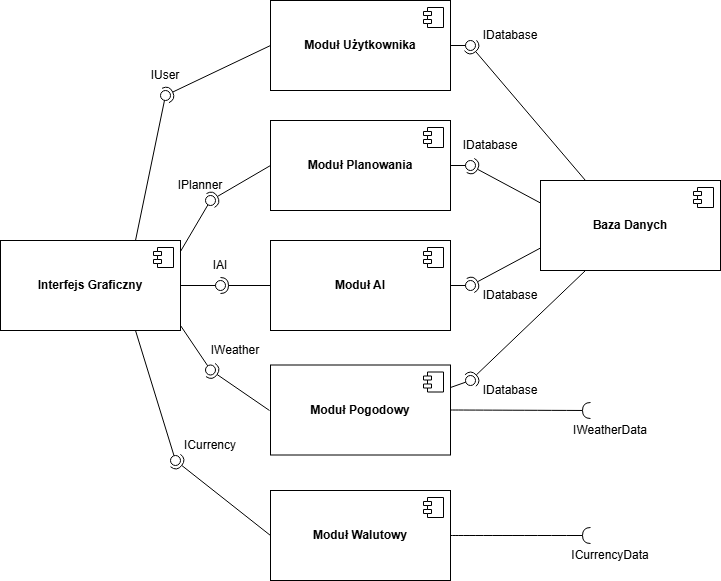
\includegraphics[width=\textwidth]{compo.png}
\caption{Diagram komponentów systemu Tripify.}
\end{figure}

\subsection{Opis komponentów}
\begin{itemize}
  \item \textbf{Interfejs Graficzny:} aplikacja kliencka pozwalająca użytkownikowi na interakcję z systemem (tworzenie i przeglądanie planów wycieczek, logowanie).
  \item \textbf{Moduł Użytkownika:} odpowiada za zarządzanie kontami, danymi profilowymi oraz procesami uwierzytelniania i autoryzacji.
  \item \textbf{Moduł Planowania:} główny komponent biznesowy realizujący układanie harmonogramów podróży.
  \item \textbf{Moduł AI:} odpowiada za integrację z zewnętrznymi modelami sztucznej inteligencji w celu analizy i budowania atrakcyjnych punktów wycieczki.
  \item \textbf{Moduł Pogodowy:} zajmuje się pobieraniem i przetwarzaniem aktualnych oraz prognozowanych informacji o warunkach atmosferycznych.
  \item \textbf{Moduł Walutowy:} odpowiedzialny za przeliczanie kosztów podróży w czasie rzeczywistym bazując na aktualnych kursach walut.
  \item \textbf{Baza Danych:} trwały magazyn przechowujący bezpiecznie profile użytkowników i wygenerowane dla nich plany.
\end{itemize}

% ====================================================
\FloatBarrier
\clearpage
\section{Diagram klas}
% ====================================================
Diagram przedstawia encje persystowane w bazie PostgreSQL przez poszczególne mikroserwisy (Auth Server oraz Backend/API Gateway) wraz z obiektami wartości (DTO) wykorzystywanymi w komunikacji.

\begin{figure}[H]
\centering
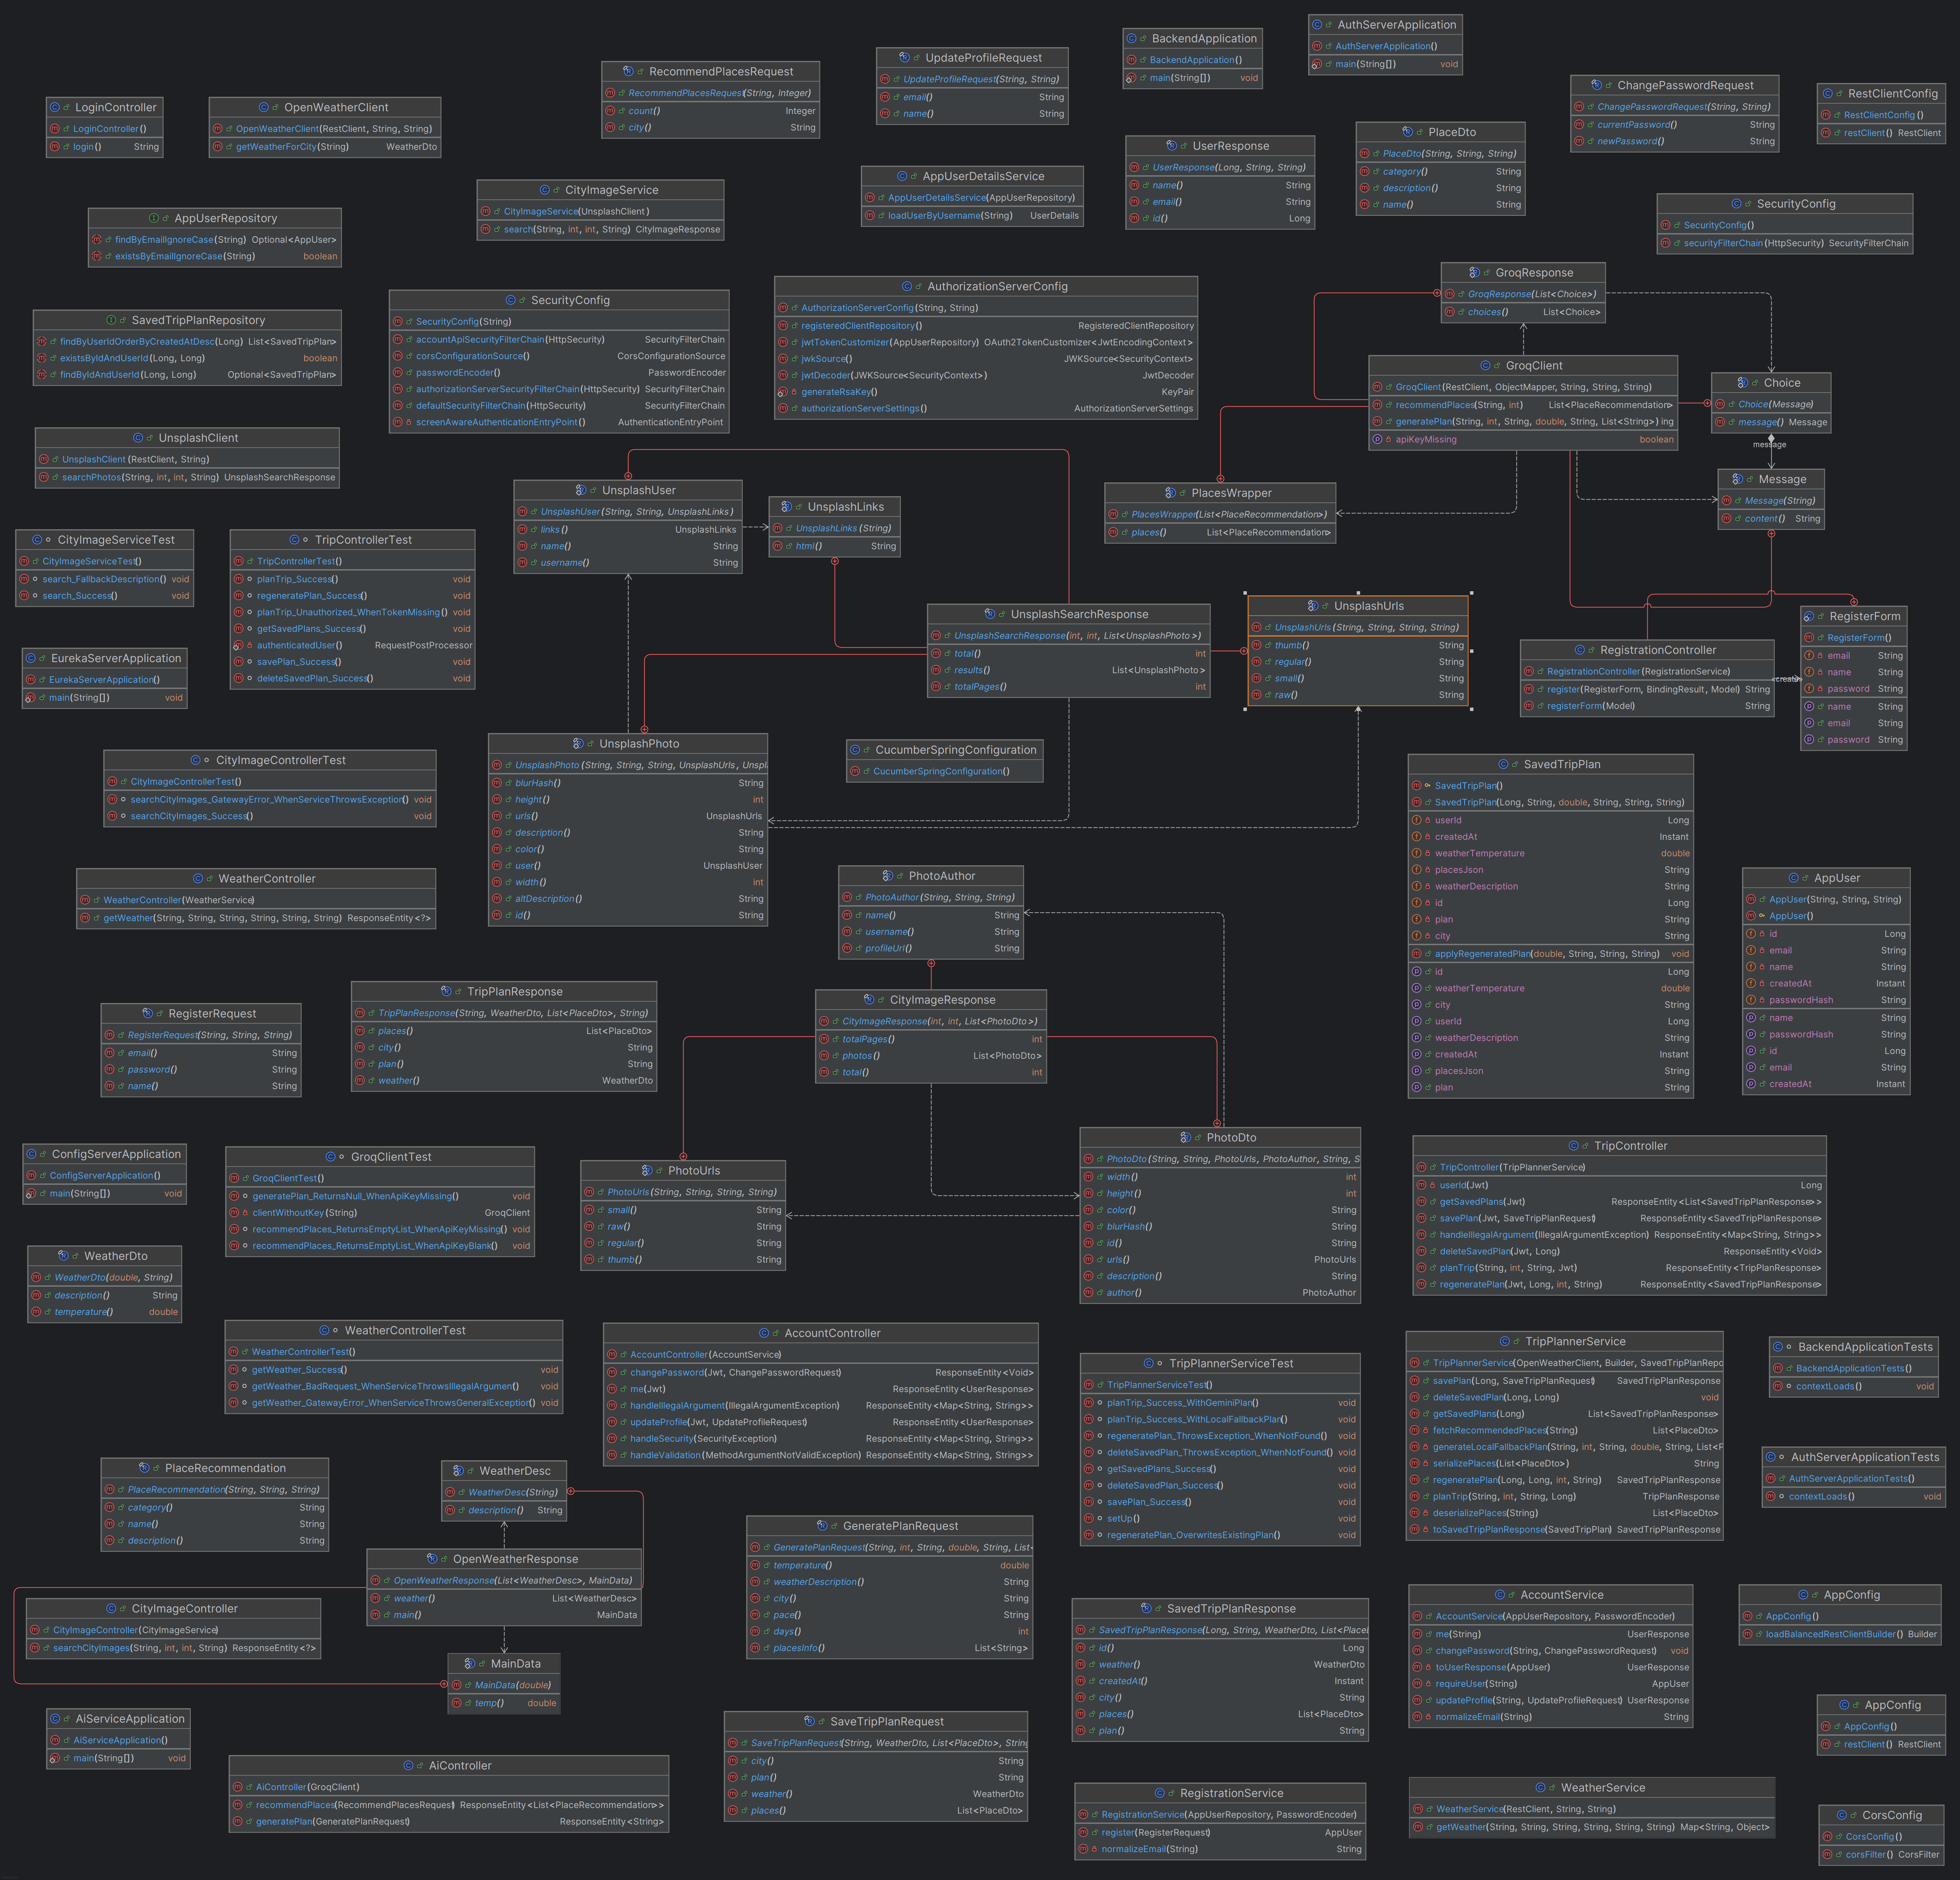
\includegraphics[width=\textwidth]{class.png}
\caption{Diagram klas systemu Tripify.}
\end{figure}

% ====================================================
\FloatBarrier
\clearpage
\section{Diagramy interakcji}
% ====================================================

% ---------- SD1: AI Plan ----------
\subsection{Diagram sekwencji: Generowanie planu wycieczki}
\begin{figure}[H]
\centering
\resizebox{\textwidth}{!}{%
\begin{tikzpicture}
\node[part] (pac) at (0,0) {Użytkownik};
\node[part] (fe)  at (3.6,0) {Frontend};
\node[part] (be)  at (7.6,0) {API Gateway};
\node[part] (ai)  at (11.4,0) {AI Service};
\node[part] (groq) at (15.2,0) {Groq LLM API};
\foreach \p in {pac,fe,be,ai,groq} \draw[dashed,midgray] (\p.south) -- (\p |- 0,-10.2);
\msg{pac}{fe}{-1.0}{podanie miasta i dni}
\msg{fe}{be}{-1.8}{POST /trips/generate}
\msg{be}{ai}{-2.6}{routing do AI Service}
\node[draw=accent,fill=white,font=\scriptsize,align=center] at (ai |- 0,-3.4) {Tworzenie Promptu};
\msg{ai}{groq}{-4.2}{POST (Prompt)}
\rsg{groq}{ai}{-5.0}{Odpowiedź w JSON}
\node[draw=accent,fill=white,font=\scriptsize,align=center] at (ai |- 0,-5.8) {Parsowanie i Zapis do DB};
\rsg{ai}{be}{-7.0}{201 Created (TripPlan)}
\rsg{be}{fe}{-7.8}{201 Created}
\rsg{fe}{pac}{-8.6}{Wyświetlenie widoku wycieczki}
\end{tikzpicture}}
\caption{Diagram sekwencji do procesu generowania planu wycieczki.}
\end{figure}

% ---------- SD2: Waluty ----------
\subsection{Diagram sekwencji: Przeliczanie walut}
\begin{figure}[H]
\centering
\resizebox{\textwidth}{!}{%
\begin{tikzpicture}
% Aktorzy i komponenty
\node[part] (pac) at (0,0) {Użytkownik};
\node[part] (fe)  at (4.5,0) {Interfejs};
\node[part] (curr) at (9.0,0) {Mikroserwis Walut (Go)};
\node[part] (nbp) at (13.5,0) {API NBP};

% Linie życia
\foreach \p in {pac,fe,curr,nbp} \draw[dashed,midgray] (\p.south) -- (\p |- 0,-13.0);

% Warunek wstępny z tabeli
\node[draw=accent,fill=white,font=\scriptsize,align=center,dashed] at (curr |- 0,-1.0) {Warunek wstępny:\\Pobrano tabele z NBP};

% Krok 1 z Głównego Przepływu
\msg{pac}{fe}{-2.2}{1. Podanie kwoty i walut}
\msg{fe}{curr}{-3.0}{Przekazanie danych}

% Krok 2 z Głównego Przepływu
\msg{curr}{nbp}{-4.0}{2. Odpytanie o kurs}

% --- PRZEPŁYW GŁÓWNY (Sukces) - Poza ramką ---
\rsg{nbp}{curr}{-5.2}{Zwrócenie kursu}

% Krok 3 z Głównego Przepływu
\node[draw=accent,fill=white,font=\scriptsize,align=center] at (curr |- 0,-6.4) {3. Przeliczenie kursów};

\rsg{curr}{fe}{-7.6}{Zwrócenie kwoty}

% Krok 4 z Głównego Przepływu
\rsg{fe}{pac}{-8.4}{4. Wyświetlenie wyniku}

% ====== BLOK ALT: Tylko dla przepływu 2a (Brak odpowiedzi) ======
\draw[accent, thick] (-1.0, -9.4) rectangle (15.0, -12.4);
\node[fill=white, font=\scriptsize\bfseries, draw=accent, thick] at (-1.0, -9.4) {ALT};
\node[font=\scriptsize\bfseries, text=accent, anchor=west] at (-0.8, -9.8) {[Brak odpowiedzi od API NBP]};

\rsg{nbp}{curr}{-10.6}{Błąd lub brak odpowiedzi}
\rsg{curr}{fe}{-11.4}{Przekazanie błędu}
\rsg{fe}{pac}{-12.0}{Wyświetlenie błędu}

\end{tikzpicture}}
\caption{Diagram sekwencji dla procesu przeliczania walut.}
\end{figure}

% ====================================================
\FloatBarrier
\section{Stack technologiczny}
% ====================================================
\begin{longtable}{p{0.20\textwidth} p{0.24\textwidth} p{0.46\textwidth}}
\toprule
\textbf{Obszar} & \textbf{Technologia} & \textbf{Uzasadnienie wyboru} \\
\midrule
\endhead
Frontend & Next.js, React & Dojrzały ekosystem, renderowanie hybrydowe
(SSR/CSR), komponentowość i wydajność;
naturalne wsparcie dla aplikacji webowej
działającej w przeglądarce. \\
\addlinespace
Główny Backend & Java 25, Spring Boot 3.x & Wbudowane rozwiązania chmurowe (Spring Cloud) w tym Eureka i Config ułatwiają obsługę mikrousług. Nowoczesne mechanizmy Javy przyspieszają rozwój. \\
\addlinespace
Mikroserwis Walut & Go (Golang) & Rozdzielenie logiki z naciskiem na wydajność i niski foot-print pamięci. Utrzymywanie w pamięci cache kursów NBP. \\
\addlinespace
Service Discovery & Eureka & Odporność i skalowalność architektury. Mikroserwisy nie muszą znać sztywnych adresów IP. \\
\addlinespace
Uwierzytelnianie & Spring Authorization Server & Standardowe i bezpieczne podejście do wystawiania własnych tokenów JWT zgodne z OAuth2. \\
\addlinespace
AI \& Obrazy & Groq API, Unsplash & Groq oferuje wyjątkowo szybkie generowanie treści LLM w stosunku do OpenAI, a Unsplash dostarcza jakościowe zdjęcia miejsc docelowych za darmo. \\
\addlinespace
Baza danych & PostgreSQL (Cloud SQL) & Relacyjna solidność w chmurze Google (GCP). Zintegrowane z Hibernate LOB. \\
\addlinespace
Konteneryzacja & Docker i Compose & Spójność środowiska developerskiego, jedno polecenie wstawia całą macierz serwerów, baz i konfiguracji. \\
\addlinespace
Jakość Kodu & SonarQube & Zautomatyzowana kontrola Clean Code'u upewniająca się o poprawnym stanie długu technologicznego. \\
\bottomrule
\end{longtable}

\section{Działanie systemu}
Poniżej przedstawiono kluczowe widoki interfejsu użytkownika systemu \sysname{} wraz z opisem ich funkcjonalności.

% ---------- Ekran logowania ----------
\subsection{Ekran logowania}
Ekran logowania umożliwia użytkownikowi uwierzytelnienie się w systemie za pośrednictwem protokołu OAuth2 z przepływem PKCE. Po podaniu adresu e-mail i hasła serwer autoryzacji weryfikuje dane i wystawia token JWT, który jest przechowywany po stronie przeglądarki. Formularz zapewnia także odnośnik do rejestracji nowego konta.

\begin{figure}[H]
\centering

\includegraphics[width=0.35\textwidth]{login.png}
\caption{Widok ekranu logowania.}
\end{figure}

% ---------- Ekran rejestracji ----------
\subsection{Ekran rejestracji}
Formularz rejestracji pozwala na utworzenie nowego konta użytkownika. Wymagane jest podanie imienia, adresu e-mail oraz hasła (minimum 8 znaków). Po pomyślnej rejestracji użytkownik jest przekierowany na ekran logowania z komunikatem potwierdzającym.

\begin{figure}[H]
\centering

\includegraphics[width=0.35\textwidth]{register.png}
\caption{Widok ekranu rejestracji.}
\end{figure}

% ---------- Strona główna ----------
\subsection{Strona główna}
Strona główna stanowi centralny punkt nawigacyjny aplikacji. Prezentuje:
\begin{itemize}
  \item \textbf{Slider popularnych kierunków} — karuzela z miastami (np.~Warszawa, Porto, Dubaj), gdzie każdy slajd wyświetla zdjęcie, aktualną temperaturę i warunki pogodowe. Kliknięcie na slajd natychmiast uruchamia generowanie planu podróży.
  \item \textbf{Przelicznik walut (NBP)} — komponent pozwalający na szybką konwersję walut w czasie rzeczywistym z wykorzystaniem kursów Narodowego Banku Polskiego.
  \item \textbf{Pole wyszukiwania} — umożliwia wpisanie dowolnego miasta i zdefiniowanie parametrów wycieczki (długość pobytu, tempo zwiedzania).
\end{itemize}

\begin{figure}[H]
\centering
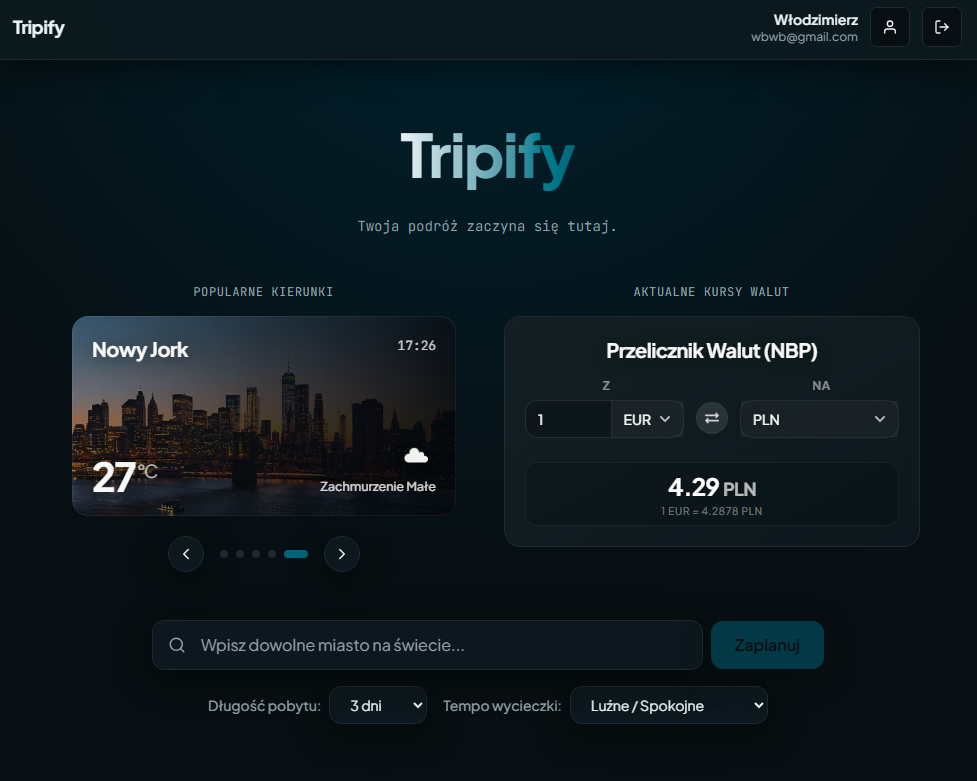
\includegraphics[width=0.85\textwidth]{home.png}
\caption{Widok strony głównej systemu Tripify.}
\end{figure}

% ---------- Wygenerowany plan ----------
\subsection{Wygenerowany plan podróży}
Po wybraniu miasta i kliknięciu przycisku ,,Zaplanuj'' system równolegle pobiera dane pogodowe (OpenWeather API), rekomendacje miejsc must-see (Groq LLM) oraz zdjęcie miasta (Unsplash API). Wynik prezentowany jest w formie:
\begin{itemize}
  \item \textbf{Baner z miastem} — zdjęcie z nakładką zawierającą nazwę miasta oraz aktualną temperaturę i opis pogody.
  \item \textbf{Lista miejsc must-see (AI)} — rekomendowane atrakcje z podziałem na kategorie (zabytek, muzeum itp.) wraz z krótkimi opisami.
  \item \textbf{Wielodniowy harmonogram} — szczegółowy plan wycieczki z podziałem na rano, popołudnie i wieczór, wygenerowany przez model AI z uwzględnieniem pogody i rekomendowanych atrakcji.
\end{itemize}
Użytkownik może zapisać wygenerowany plan do swojego profilu przyciskiem ,,Zapisz plan''.

\begin{figure}[H]
\centering
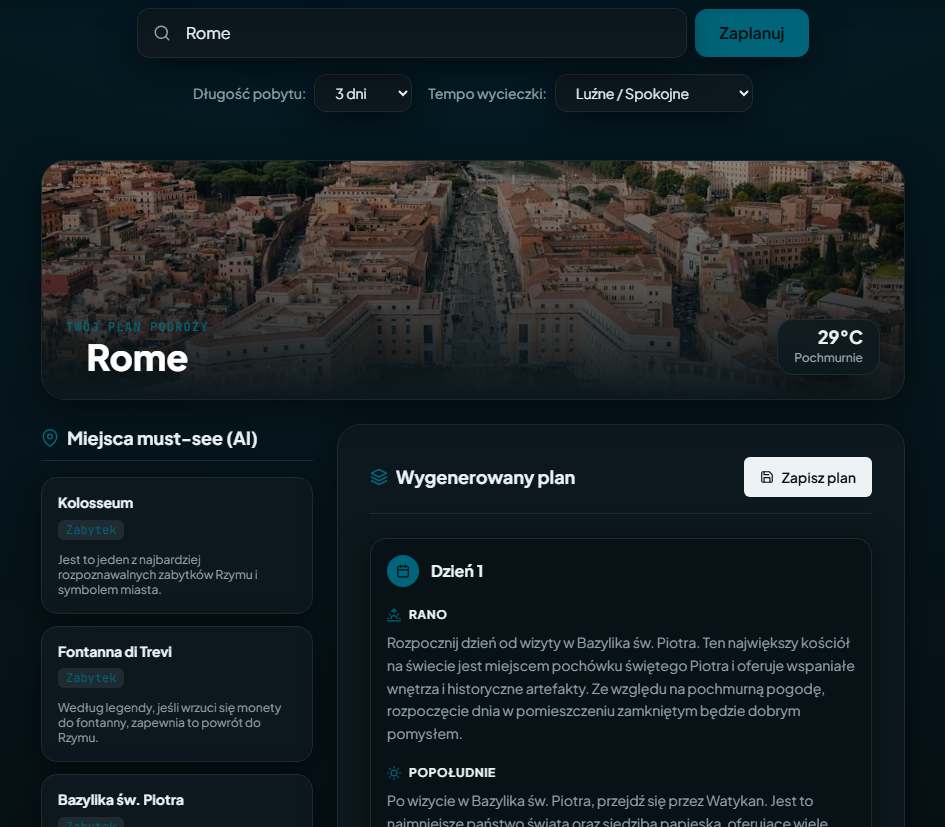
\includegraphics[width=0.85\textwidth]{plan.png}
\caption{Widok wygenerowanego planu podróży dla miasta Rzym.}
\end{figure}

% ---------- Panel użytkownika ----------
\subsection{Panel użytkownika}
Panel użytkownika umożliwia zarządzanie kontem oraz zapisanymi planami podróży. Zawiera trzy sekcje:
\begin{itemize}
  \item \textbf{Dane konta} — edycja imienia oraz adresu e-mail.
  \item \textbf{Zmiana hasła} — formularz do bezpiecznej zmiany hasła z polem potwierdzenia.
  \item \textbf{Zapisane plany podróży} — lista wcześniej wygenerowanych planów z podglądem miasta, daty utworzenia, temperatury, rekomendowanych miejsc oraz możliwością rozwinięcia pełnego planu, regeneracji z nowymi parametrami lub usunięcia.
\end{itemize}

\begin{figure}[H]
\centering
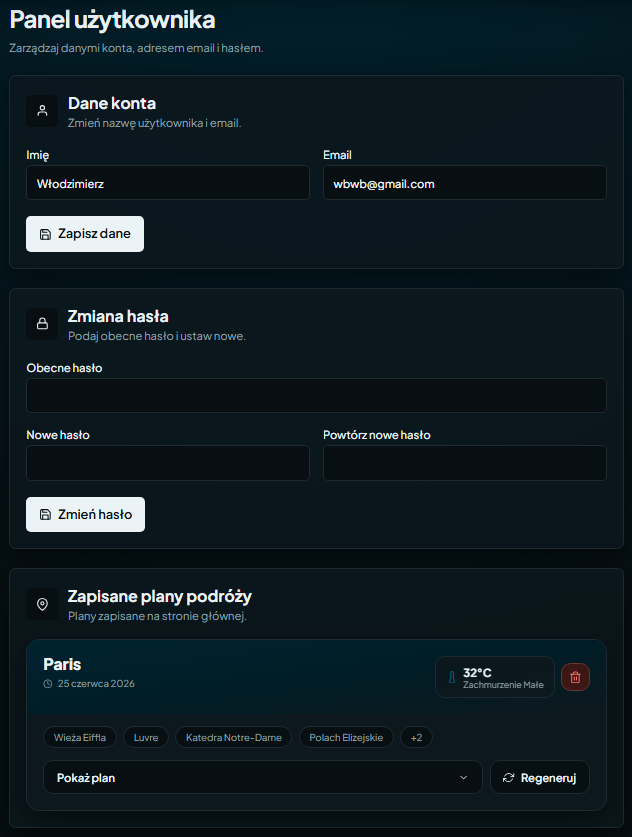
\includegraphics[width=0.65\textwidth]{user_panel.png}
\caption{Widok panelu użytkownika z zapisanymi planami podróży.}
\end{figure}

% ====================================================
\section{Podsumowanie}
% ====================================================
Architektura aplikacji \sysname{} reprezentuje nowoczesne podejście do złożonych projektów programistycznych poprzez zastosowanie spójnego i dobrze zorganizowanego wzorca \textbf{Mikrousług}. Zamiast pojedynczego monolitu system posiada specjalizowane serwisy: do autoryzacji (Auth Server), orkiestracji (API Gateway), generowania planów (AI Service) czy przeliczania walut (Currency Converter). Dzięki wdrożeniu \textbf{Eureka Server} i \textbf{Config Server} zarządzanie tą złożonością pozostaje przewidywalne i gotowe na skalowanie.

Wykorzystanie zewnętrznych usług — takich jak model \textbf{LLM z Groq}, API pogodowe czy zdjęciowe — pozwala niewielkim kosztem stworzyć ogromną wartość dodaną dla podróżnika, dając mu komplet informacji podczas jednej sesji logowania. Projekt został przygotowany we współpracy z systemami kontroli jakości (SonarQube) oraz jest w pełni konteneryzowany (Docker). Taka architektura jest wysoce skalowalna i otwarta na dodawanie nowych modułów, stanowiąc stabilny fundament dla inteligentnego systemu wspomagania podróży.
\end{document}
